\begin{bibunit}
\thispagestyle{plain}

% Add missing command definitions from original paper
% \texttt is already defined in LaTeX, so we don't need to redefine it

\section*{Abstract}
    IEC 61499 is an executable, event-based language for control software that allows visual and textual implementation of individual software components (Function Blocks, FBs). The standardized visual service sequence model specifies the expected input/output behaviour of a component, thus supporting model-based testing. We present our approach for testing an FB on various platforms, which helps manage the variations in execution semantics between different vendors. First, service sequences are generated manually or derived from an existing (partial) implementation. Then, these service sequences serve as unit tests for this implementation. Finally, we create a test application that is executable on any IEC 61499-compliant platform. Executing tests directly in the target platform helps validate the correct functionality of an FB before deploying the control software to a cyber-physical system. 

\section{Introduction}

In industrial settings, Programmable Logic Controllers (PLCs) coordinate mechatronic components, each equipped with a control program. Interactions between the individual programs form an emergent system, i.e., a distributed control system. However, current control systems are highly dependent on specific vendors, hindering the transfer of programs between different platforms. As seamless integration is a key requirement in the context of Industry 4.0, this lack of interoperability poses great challenges.

The IEC 61499 standard \cite{61499} addresses the issues of vendor lock-in and offers a solution by providing a framework for developing portable and interoperable software. Although the file exchange format is standardised, it is currently interpreted differently and the execution semantics varies among vendors \cite{christensen.2012,Thramboulidis.2009}. As a result, migrating programs from one IEC 61499 platform to another, and thus executing them in a different run-time environment (RTE), may introduce errors that are difficult to detect but could lead to damage to humans or the physical equipment \cite{Testing_Midhun}. Therefore, it is crucial to thoroughly test an IEC 61499 application on the target platform before deploying it to a real-world system. A platform-independent test specification has the potential to greatly reduce the involved effort.

Unit testing is a fundamental approach in software testing, which evaluates the implementation of a piece of software \cite{softwareTesting} to ensure its reliability. In IEC~61499, executing a test requires providing event and data signals. For control engineers who develop Function Blocks (FBs), it can be challenging to manually create a test FB and the required test application for observing the results. Model-based testing can reduce the manual effort and also supports a ``test first and fail'' methodology, known as Test-Driven Development (TDD) \cite{hametner2014}, which is widely used in agile software engineering.

Previous work showed the feasibility of using service sequences as test specifications \cite{wiesmayr2021,hametner2014}. 
Existing testing mechanisms require dedicated tool support and cannot be directly transferred to other platforms. The portability of IEC 61499 software allows migrating applications to other IEC 61499 vendor platforms, but ensuring that a program behaves consistently across RTEs remains an open challenge. 
In this paper, we therefore present our approach for testing FBs that allows to execute tests on any IEC 61499-compliant RTE. Based on test scenarios that are created as a service sequence model, we generate the corresponding test application. %FB, establish the necessary connections with the FB under test, execute each test scenario, compare the results, and provide the test outcome. 
Realised as a composite FB, the test application is portable across various IEC 61499 platforms and allows for validating the correct functionality before deployment in real-world machinery. We present an example (Section III), the methodology (Section~IV) and our proof-of-concept implementation (Section V).

\section{State of the Art}
Developers can apply various testing strategies prior to deploying an application. They can be differentiated based on the involved software activities (e.g., unit tests or integration tests), the maturity of the software, and the degree of automation~\cite{softwareTesting}. 

Simulation techniques such as visualisations or Digital Twins are commonly employed to assess whether a control application operates according to the intended logic. However, relying on a simulation does not ensure correctness, as some malfunctions may occur only on a PLC. Finally, simulations can also aid in comprehending the system's behaviour.

The approach presented in \cite{Testing_Midhun} for creating a test suite with IEC~61499 FBs allows systematically evaluating the portability between RTEs. In this paper, we adapt this concept to test FBs in a platform-independent test application. 

Like testing, formal verification can be used to enhance the system's reliability by checking various properties. Formal verification does not require any RTE. Sinha et al.\,\cite{Sinha.2019} provide an overview of formal methods for IEC~61499. Formal verification may uncover errors that do not occur during simulations, thus, identifying certain undesirable situations. 
Verification and testing can complement each other \cite{Hussain.2006}. During the development, tests provide an early feedback, even if the model is still incomplete. Furthermore, errors that are introduced by the compiler may lead to runtime issues, but might not be revealed by formal methods. 

\subsection{Test Strategies for Unit and Functional Testing}
Verification techniques and many testing strategies are employed after developing the control program. To mitigate errors and fulfil the requirements of each FB, it can be beneficial to integrate testing approaches already into the system design phase (e.g., TDD). Unit testing ensures that each FB meets its specified requirements. After developing the control program for the entire system, functional testing can be conducted. This involves assessing the control system by providing input data and verifying the output against expected results.
Two distinct testing strategies can be applied. Their integration into the IEC 61499 development is covered in the next sections. 

\subsubsection{Approach A: Manually Create Test FBs}
Previous work has demonstrated an approach for manually creating test FBs \cite{Testing_Midhun} for an IEC 61499 FB with control logic. These test FBs encompass multiple test scenarios and embed the control logic. The expected result is compared with the result obtained from executing the control logic. A test FB is implemented as a Basic FB with event and data pins. Each input event represents a test scenario linked to specific data inputs, while output events indicate the expected result and corresponding data outputs. When a test scenario is triggered, the state diagram (i.e., Execution Control Chart, ECC) executes an algorithm that assigns input values, generates outputs based on those values, and triggers the output event.

\subsubsection{Approach B: Automatically Generate Test FBs from Specification Models}
Tools should support engineers in specifying test cases to reduce the required software engineering knowledge and increase efficiency \cite{hametner2014}. Model-based testing involves automating at least part of the testing activities. For IEC~61499 FBs, service sequences are suitable for specifying tests \cite{hametner2014}. 
% TODO describe here in related work existing work on model-based testing or sth like that?? shift our new work to the beginning of the next section
A test runner can execute these tests in an RTE and automatically evaluate the results \cite{hametner2014}. Additionally, executing models directly can allow feedback without involving any RTE and is also feasible for service sequences \cite{wiesmayr2021}. The former approach requires specific tool support for a certain RTE, the latter cannot provide feedback regarding issues introduced in the deployment to an RTE. Our approach builds upon these works. 
As an alternative to service sequences, UML models have been used as test specifications \cite{Hussain.2006}. From a state-based model, test cases can be derived using coverage-driven algorithms \cite{Hussain.2006}. Using an evolutionary algorithm, test cases with a high coverage were generated directly from the FB model in \cite{Buzhinsky.2015}. Test case generation can augment our approach, which focuses on executing tests of any source on multiple platforms. Additional tool support would be however required to use other kinds of test specifications.
%In this approach, a test specification is created as service sequences to test the developed IEC 61499 function block with control logic. However, this approach is executed in the interpreter and does not have runtime support. The results are compared to the output of the sequence primitive.


\subsection{Identified Issues Regarding Platform Independence}
Two major problems are associated with distributed control software that spans multiple platforms: 
(i) The \emph{lack of automated tool support for RTE comparison} makes comparing the behaviour and performance of FBs across different RTEs a challenging task. Currently, manual comparison is time-consuming and error-prone. Dedicated tools should analyse and evaluate the behaviour of FBs in different RTEs to ensure accurate comparison.

(ii) \emph{Software development for different RTEs} is challenging because the compatibility and portability of an FB across different RTEs cannot be assumed. 
For example, if an FB is initially developed and tested on one RTE, such as NXT EcoRT, there might be a need to reuse that FB in another project in a different RTE, such as 4diac FORTE. Differences in RTE behaviour, programming languages, and underlying architectures can cause compatibility issues and hinder the seamless transfer of FBs between different RTEs. 

\section{Running Example: Simple Calculation FB}
Our running example (Fig. 1) is an alternative addition FB that calculates the output based on the inputs according to the formula \texttt{DO1:=DI1+2*DI2}, with the following elements:

\begin{figure}[htbp]
    \centering
    \vspace{-5mm}
    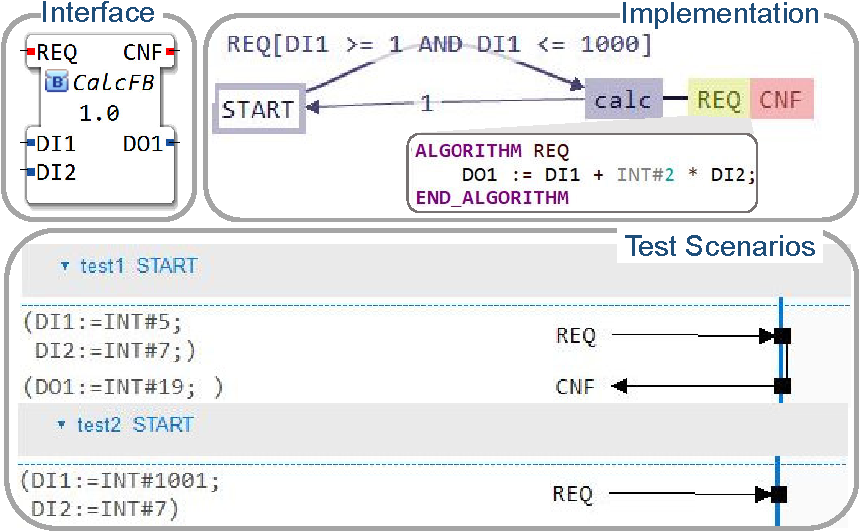
\includegraphics[width=0.95\columnwidth]{MX_Papers/Paper9/Figures/running_example-crop.pdf}
    \caption{Running Example: FB performing simple calculation. FB interface defining the component, implementation as state diagram, and two usage scenarios modelled as service sequences.}
    \label{fig:running_example}
\end{figure}
\begin{figure*}[htbp]
	\centering
	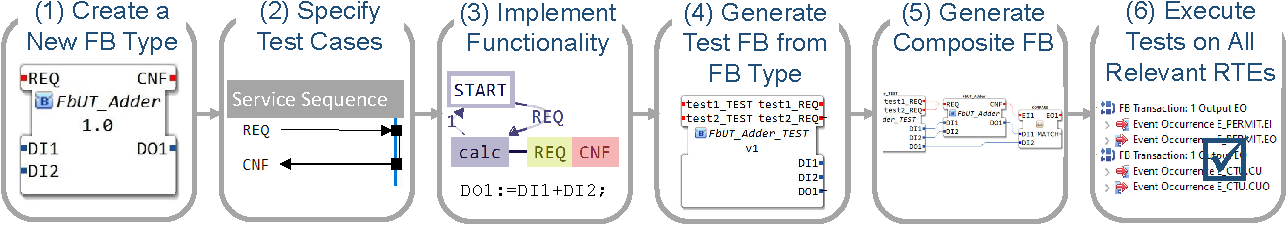
\includegraphics[width=1\textwidth]{MX_Papers/Paper9/Figures/process-crop.pdf}
	\caption{Overview of process for testing FBs across various software platforms. }
	\label{methodology}
    \vspace{-5mm}
\end{figure*}
\begin{itemize}
   \item Input event \texttt{REQ} triggers the calculation.
   \item Data inputs \texttt{DI1}, \texttt{DI2} are used for the calculation. They receive values from external sources or other FBs.
   \item Data output \texttt{DO1} stores the result of the calculation performed by the FB.
   \item Output event \texttt{CNF} is issued to indicate the completion of the algorithm execution and the availability of the result. Sending this event indicates that the output result is ready to be used or transmitted to other FBs.
   \item Algorithm \texttt{REQ} within the FB is executed when the input event \texttt{REQ} occurs. It performs the calculation using the input variables \texttt{DI1} and \texttt{DI2}.
   
%The algorithm statement DO1 := DI1 + 2 * DI2 assigns the result of the calculation to the output variable DO1.
%Once the algorithm execution is completed, the function block triggers the CNF event to indicate that the output result is ready to be used or transmitted to other function blocks.
\end{itemize}

In our example, the FB performs the calculation if the values of \texttt{DI1} and \texttt{DI2} are between 1 and 1000 (cf. state diagram in Fig. 1). When triggering the \texttt{REQ} event with appropriate input values, the FB executes the algorithm and produces the respective output. 
%\subsection{Running Example: Service Model}

In the running example, a service model is provided to define the test scenarios for the FB (cf. Fig. 1). The service model specifies the expected event occurrences, as well as the input values (\texttt{DI1} and \texttt{DI2}) and the expected output value (\texttt{DO1}) for each test case. 
Let us discuss the two test scenarios,  \texttt{test1} and \texttt{test2}. 
The scenario of \texttt{test1} is triggered upon arrival of an event at the input \texttt{REQ}. The purpose of \texttt{test1} is to verify the FB behaviour by checking whether it correctly returns 19 when given input values of 5 and 7. 
% Test 1: 
% \begin{itemize}
%    \item For test1, the input values are:
% - DI1 is assigned the integer value of 5 (INT 5).
% - DI2 is assigned the integer value of 7 (INT 7).
% 
%    \item The expected output value is:
% - DO1 is expected to have the integer value of 19 (INT 19).
% 
% \end{itemize}
% 
% 
% 
% 
%     Test 2:
%     
%     \begin{itemize}
%        \item For test2, the input values are:
%     - DI1 is assigned the integer value of 9 (INT 9).
%     - DI2 is assigned the integer value of 5 (INT 5).
%     
%        \item The expected output value is:
%     - DO1 is expected to have the integer value of 19 (INT 19).
%     \end{itemize}
Similarly, \texttt{test2} aims to verify the FB behaviour for an edge case, as one value will be out of range (i.e., \texttt{DI2:=INT\#1001}). We expect that no addition is performed, and no output events are sent (cf. second sequence in Fig.~1). 
In both test cases, the expected output value is explicitly specified. By comparing the actual output with the expected output for each test case, the implemented FB behavior can be evaluated.%it can be determined whether the FB behaves as intended.
% TODO BIANCA adds the figures to this sequence


\section{Proposed Methodology for Testing FBs}
Our proposed approach consists of several steps regarding creating test cases, generating test applications, and executing a test application on various RTEs (cf. Fig. \ref{methodology}). Detailed transformation rules will be described in the next section.

\subsubsection{Create a New Function Block Type (FBT)} The FB implements the desired functionality. This involves specifying the input/output events and data inputs/outputs. Unless the developer adheres to a TDD process, the internal behaviour of the FB is implemented as well.

\subsubsection{Specify Test Cases as Service Sequence Models} Models are specified manually or with tool support. Manually defining service sequences allows a TDD process. Either the standardised XML is edited directly, or graphical editors are used. For existing implementations, using a model execution framework allows recording service sequences with tool support as described in \cite{wiesmayr2021}. Recorded tests can serve as regression tests, as they capture the actual behaviour of an executed FB.

   %In this step, the test cases for the FB are specified as service models. There are two approaches to this:
   % \begin{enumerate}
   % \item Manually defining Service Sequences: The test cases are manually defined as service sequences, representing the expected behaviour of the FB under different scenarios.
  %  \item  Recording Service Sequences using the interpreter: Alternatively, the test cases can be recorded using the interpreter, which 
 %   \end{enumerate}

    \subsubsection{Implement Functionality}
    When following a TDD process, the functionality of the FB is implemented at this stage. The specified tests can be used for evaluating the correctness.
   
  
\subsubsection{Generate Test FB from FB Type Specification}
    An IEC~64199-compliant test application can be ported to various RTEs.
   Based on the specification of the FB under test, and the information provided by the service models, a test FB is generated. This test FB incorporates the expected results of the FB under test and is configured to execute the specified test cases upon receiving a trigger event.
   
\subsubsection{Generate Composite FB to Evaluate Results}
  This FB connects the test FB of step 4 with the FB under test. 
   Additional FBs can capture the results for each test case.
   
\subsubsection{Execute Tests in All Relevant RTEs}
   The generated test application (i.e., the composite FB), is deployed to and executed on different RTEs. The behaviour and output results of the FB in each RTE are evaluated.

Sophisticated tool support can automate a large part of the process, especially regarding the steps 4 to 6. By following this methodology, control engineers can effectively test new FBs. The systematic approach ensures that FBs are thoroughly tested for functionality and compatibility across various RTEs.

\section{Implementation}
Based on the instructions provided in \cite{Testing_Midhun}, we derived transformation rules for automatically generating test FBs. Then, we implemented these rules as a proof-of-concept in an IDE for IEC 61499-software.

% TODO: one output event per sequence, not in general
% TODO: WITH for the triggering events
% TODO: one state per sequence only if sequence has single input event
% 
% \begin{figure}[!t]
% 	\centering
% 	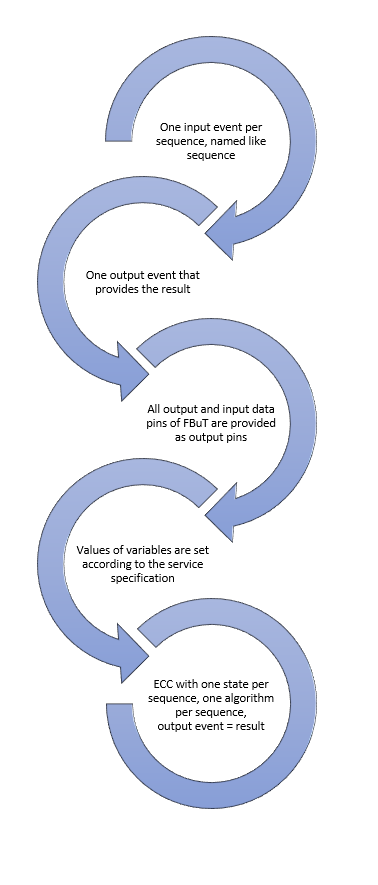
\includegraphics[width=0.25\textwidth]{MX_Papers/Paper9/Figures/Trules.PNG}
% 	\caption{TransformationRules}
% 	\label{TransformationRules}
% \end{figure}
\subsection{Transformation Rules}
The test FB for the platform-independent test application is created according to the following initial set of guidelines. 
We will explain each transformation rule for constructing the test FB in detail, while referring to our running example. The resulting test FB is shown in Fig. \ref{fig:testfb}.

\begin{figure}[htbp]
    \centering
    \vspace{-5mm}
    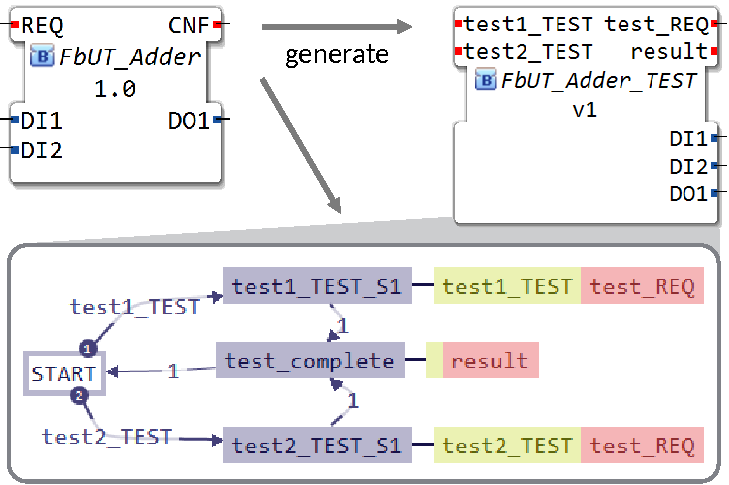
\includegraphics[width=\columnwidth]{MX_Papers/Paper9/Figures/testFB-crop.pdf}
    \caption{Creating test FB for an FB under test. The behaviour of the test FB is implemented as a state diagram (Execution Control Chart, bottom Figure).}
    \label{fig:testfb}
\end{figure}

\subsubsection{One Input Event per Service Sequence}
Every service sequence must result in a corresponding input event at the test FB. The name of the input event should reflect the one of the realised service sequence to show their association. %be chosen to accurately reflect its association with the respective sequence, thus, facilitating identifying the triggered sequence. 

\subsubsection{One Output Event per Input Event of FB under Test}
The test FB will trigger all required events that are part of a test sequence. As a result, the test FB requires one output event for each input event of the FB under test. 

\subsubsection{One Output Event for Triggering the Comparison}
There should be a single output event in the test FB that represents that a test sequence was completed (named \texttt{result}).

\subsubsection{One Data Output per Data Pin of the FB under Test}
This rule specifies that all input and output data pins of the FB under test should be exposed as output pins in the test FB. These outputs are used for instrumenting the FB under test and for the comparison.

\subsubsection{Values of Variables Are Set According to the Service Specification}
The values of the data outputs from the previous step should be set based on the service sequence specification, which defines the input values and expected output values for each sequence. We assume that values for all data pins are present in the service sequence model for careful monitoring of the data flow. %Setting the variables accordingly ensures that the service model accurately represents the desired behaviour of the function block.

\subsubsection{State Diagram of Test FB Has One State per Transaction}%Execution-Control-Chart (ECC) with one state per sequence, one algorithm per sequence}
There should be one state in the state diagram of the test FB per transaction of the sequence. Each specified input event in a service sequence starts a new transaction. Each state has an algorithm which updates the data outputs. Sending an output event is required to publish these data values.

\subsubsection{Output Event Occurrence upon Completing Test}
In Rule~3, an output event pin was defined for completing the sequence. The state diagram has to ensure that this event is sent after completing a sequence.
%The final transformation rule states that the output event of the service model should be designated as the event that provides the result. This output event is responsible for transmitting the calculated or derived value as the final result of the service sequence, as specified in the service model.
%By adhering to these transformation rules, the service model for the function block can be structured consistently and systematically, ensuring clarity, ease of understanding, and effective testing of the function block's behaviour.
The generated test FB is part of a test application. We created a composite FB manually in Fig. \ref{fig:compfb} (according to step 5 in Section~IV).
\begin{figure}[htbp]
    \centering
    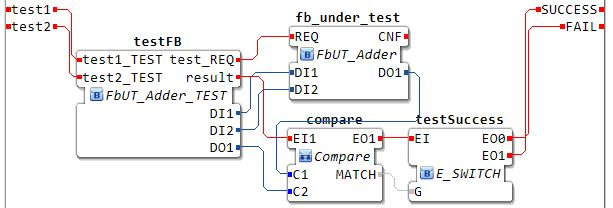
\includegraphics[width=\columnwidth]{MX_Papers/Paper9/Figures/compositeFb.JPG}
    \caption{Composite FB encapsulating the test application. The FB under test receives event and data signals from the test FB, which realises the test cases from the service sequence model.}
    \label{fig:compfb}
\end{figure}
\subsection{Tool Support}
Tool support for specifying service sequences and simulating their results is available in Eclipse 4diac \cite{eclipse4diac} from previous work \cite{wiesmayr2021}. We have extended the tool with a test FB generator, which uses the information provided in service models to create test code. With respect to the proposed process (Fig.~\ref{methodology}), we focused on automating step~4 in this proof-of-concept implementation. Furthermore, not all service sequence models are supported at this stage. For instance, a scenario comprising different events in a single test cannot be used as a source for automatically generating a test FB yet.

\section{Conclusion and Future Work}
In conclusion, the proposed testing methodology for IEC 61499 FBs offers systematic and reliable means to verify the correct behaviour of FBs across diverse RTEs. The generation of test FBs from a model-based specification, represented as a service sequence, was accomplished through semi-automated means. Engineers can manually create the test specification (e.g., for test-driven development), or derive it from an existing implementation via the IDE. Our created test FBs are portable across platforms to allow platform-independent testing. This paper presented the overall approach and a first proof-of-concept implementation. We provide an initial set of transformation rules and the corresponding tool support for automating part of the process.

In future work, we aim to support all kinds of FB implementations, provide also the test applications automatically, and evaluate our approach based on a realistic use case to evaluate the scalability and feasibility of the approach in practice. Additionally, developing a runtime comparison tool to analyse and compare the behaviour and performance of FBs across different platforms would enable control engineers to identify and address discrepancies. Finally, integrating the testing approach with further model-based development techniques, such as formal methods or simulation, would provide a holistic approach to system verification and enhance the overall reliability of developed systems.

\clearpage
\putbib
\end{bibunit} 